% Appendix F: details of Claim 3 (where an intervention appears to act). Input by sections/appendix.tex.
\section{Where an intervention appears to act: details}\label{app:claim3}

This appendix gives the design and every result of the final round's test of the channel-ratio law (preregistration J, part C): five families of identity edits obtained independently of the natural clamp, in Qwen2.5-7B, Mistral-7B and Llama-3.1-8B, on 80 new stories (\cref{app:prompts-intervention}). The motivating case, the released remap, is in \cref{app:remap}; the binding swap at block 28 and the overlap screen are in \cref{app:binding-j}. % verbatim: 80 stories, entry J part C

\subsection{The law, the lemma and the statistics}\label{app:law}

\paragraph{The law.} For an edit $Z$ that writes a value at the writing token at depth $l$ (the output of 0-based block $l$), channel $C \in \{K, V, KV\}$ and format $f$, let $\psi_C^Z(f, l) = \overline{\mathrm{ID}}{}_C^Z / \overline{\mathrm{ID}}{}_C^{\mathrm{nat}}$ be the edit's identity effect through channel $C$ as a share of the natural write's, from block $l{+}1$ on. The channel-ratio law states that one scaling per edit holds for both channels and in every format: $\psi_K^Z = \psi_V^Z$. Its statistic is $\lambda = \log(\psi_K/\psi_V)$ (\cref{sec:claim3}; each $\psi$ floored at 0.01, so that a dead channel is a departure), computed in three ways at each depth: $W(f, l)$ within one format, for \fmtOpt{} and \fmtPost{} where both channels are used; $A_L(l)$, the key read under \fmtLetter{} against the value read under \fmtNone{}; and $A_P(l)$, the key read under \fmtOpt{} against the value read under \fmtNone{}. A channel is used in a cell when its natural identity effect is at least 2 nats and at least a tenth of the joint effect. A statistic is equivalent when its 90\,\% interval lies inside $\pm\log 1.25$ (two one-sided tests at 5\,\%); it counts as a departure when the edit's key and value effects interact (its interaction $\iota_{KV} > 0.5$ in one of its cells; not the $\iota$ of \cref{app:flag}). The law holds in a combination of model, edit and depths (a combo) when it has at least three statistics and every one is equivalent; otherwise the combo's pattern is copy-only (rival R1: pooled $\bar\lambda \leq \log 0.5$), key-flat (R3: $\bar\lambda \geq \log 2$) or a graded departure. A line over several combos holds only if every evaluable combo holds (an intersection-union test).

\paragraph{The lemma.} Because the base and source prompts differ only at the writing token $p$, an edit confined to the residual at $(p, l)$ reaches every other position only through $p$'s keys and values in blocks $\geq l{+}1$: under the causal mask $p$'s residual reaches other tokens only through attention, and $p$'s keys and values in blocks $\leq l$ are computed from inputs the edit does not change. So the base run with the edit's keys and values written at $p$ from block $l{+}1$ is exactly the edited run, and its key-only and value-only rows are exact. Writing the source run's residual $h_{\mathrm{S},l}(p)$ gives the source's keys and values at $p$ from $l{+}1$: this edit is the natural clamp itself. Every edit is therefore applied as a clamp row whose tables come from a prefix pass with the edit written; the prefix through $p$ is the same in all four formats, so an edit's tables are the same tensors in every format and only the readers after $p$ differ. The unit tests check the lemma in FP32 to $10^{-4}$.

\paragraph{Controls of the design.} The natural write written as an edit (T) is the equivalence control: its tables and rows equal the natural ones bitwise in every evaluable cell of all three models (\JcGoneCellsQwenSeven{} cells each), so every statistic of T is equivalent. A sensitivity gate checked that the statistics can see a departure: synthetic rows whose key table is interpolated halfway toward the base run (SK50) were classified as copy-only ($\bar\lambda$ = \JcGeightSkFiftyQwenSeven{}, \JcGeightSkFiftyMistralSeven{} and \JcGeightSkFiftyLlamaEight{}), and rows with the value table halved (SV50) as graded departures (\JcGeightSvFiftyQwenSeven{}, \JcGeightSvFiftyMistralSeven{}, \JcGeightSvFiftyLlamaEight{}). The design's earlier key-share rule ($\kappa = K/(K+V)$ within a margin of the natural share) passes SV50, a two-fold channel departure: this compression is why the law is stated on log ratios. The natural format effect on the key share is large in all three models ($\sigma(\text{\fmtLetter{}}, 3) - \sigma(\text{\fmtNone{}}, 3)$ = \JcGtwoQwenSeven{}, \JcGtwoMistralSeven{} and \JcGtwoLlamaEight{}). Intervals of the law are 90\,\% hierarchical bootstrap intervals over the 24 ordered base--source pairs and the stories within them (with the remap's two seeds as a further level); others are 95\,\%. % verbatim: entry J part C

\subsection{The edit families and their gates}\label{app:edits}

\paragraph{Families.} Each edit writes, at $(p, l)$ for $l \in \{3, 7, 11, 15\}$, a target value $t$ (S or X) in place of B:
\begin{itemize}\setlength\itemsep{0pt}
  \item \textbf{E1}, in-task steering vectors: $h_{\mathrm{B}} + \mu_1(t) - \mu_1(\mathrm{B})$, with $\mu_1(x)$ the mean residual at $(p, l)$ over 150 held-out stories with $x$ written \citep{turner2023actadd,panickssery2023caa};
  \item \textbf{E2}, steering vectors from unrelated sentences: the same with $\mu_2(x)$, the mean block-$l$ output at the token of $x$ over 24 neutral sentences;
  \item \textbf{E3}, features of a public sparse autoencoder (Qwen2.5-7B only): the BatchTopK dictionaries of \citet{andyrdt2025saes} \citep{bussmann2024batchtopk} at layers 3, 7, 11 and 15, at a pinned revision; the edit sets the latents most selective for $t$ to their mean on stories with $t$ written and removes those selective for B, leaving every other latent and the reconstruction error at B's; the number of latents (\JcGthreeKfThree{} at every layer) was set on calibration stories;
  \item \textbf{E4}, a remap trained at the writing token: a rank-16 distributed alignment search basis fitted at $(p, l)$ with the released training recipe of \citet{anonymous2026fitted} (pair-swap objective, six-way cross-entropy, one epoch over 1{,}000 training stories, two seeds, one from the PCA basis and one random), without a later mention; its losses fell from \JcDasLossFirstMin{}--\JcDasLossFirstMax{} to \JcDasLossLastMin{}--\JcDasLossLastMax{} and its held-out flip rates are \JcDasFlipMin{}--\JcDasFlipMax{};
  \item \textbf{E5}, the boundary family: steering vectors that write $t$ as its French (FR) or German (DE) word or a synonym (SYN), and the part of E1 outside the English lexical span (NL); scaled by 1 or 2 on calibration stories.
\end{itemize}
Each edit's displacement is split into its component along the story's natural displacement (PAR) and the rest (PERP), and into its projection on the five-dimensional span of the English candidate words' mean residuals (LEX) and the rest (NONLEX). A component carries identity when its effect without a later mention is at least 0.3 of the natural one with a lower bound above zero. The distance $\nu$ of an edit's cached keys and values from the natural ones, relative to the natural displacement, is reported per cell (post hoc use in \cref{app:nu}). % verbatim: entry J part C

\paragraph{Gates.} The FP32 tests passed (95 tests). T reproduced the natural tables in every evaluable cell; the natural format effect held; the sensitivity gate held in all three models. The cell gate (natural joint effect at least 2 nats, interaction at most 0.5, coverage at least 0.8) failed in \JcGfourFail{} of 48 cells: \fmtLetter{} at blocks 11 and 15 in every model, where the natural effect is small. The efficacy gate (flip rate at least 0.8 of the natural and $\varphi$ above 0.5 without a mention) held for E1 and E2 at every depth in all three models ($\varphi$ \JcGfivePhiNearMin{}--\JcGfivePhiNearMax{}) and for E3 at all four layers (\JcGfivePhiEthreeMin{}--\JcGfivePhiEthreeMax{}); E4 is effective at blocks 3 and 7 at Qwen2.5-7B and 3, 7 and 11 at Mistral-7B ($\varphi$ \JcGfivePhiEfourEffMin{}--\JcGfivePhiEfourEffMax{}) and not deeper; the E5 sub-families are mostly ineffective. Random directions of the natural norm move nothing beyond the specificity bound at any depth. % verbatim: outcome J part C

\paragraph{The dictionary gate failed through its specification.} The gate required each dictionary's fraction of variance explained (FVE) on its block's outputs, over every prompt position after the first, to be within 0.05 of its published value. It failed at all four layers (FVE $\JcGthreeFveRoundThree$, $\JcGthreeFveRoundSeven$, $\JcGthreeFveRoundEleven$ and $\JcGthreeFveRoundFifteen$ against published values of \JcGthreePubRoundThree{}, \JcGthreePubRoundSeven{}, \JcGthreePubRoundEleven{} and \JcGthreePubRoundFifteen{}), so E3 is not evaluable in every line that uses it. The published FVE is computed after the dictionary's training buffer drops the first tokens of each sample and activations with norms above ten times the batch median; the gate dropped only the first position and kept the chat template's tokens, identical in all prompts, where large-norm activations appear from block 3 on (inferred: the layer-3 dictionary explains \JcGthreeFvePrevThree{} of the variance on block 2 and fails on block 3; the per-position activations were not saved). At the writing position the layer-3 dictionary reproduces its published value (FVE \JcGthreeFvePThree{} against \JcGthreePubRoundThree{}), and E3 flips every answer at every layer. The gate measured reconstruction over positions that the dictionary's published fit excludes; a corrected gate needs a rerun. After the data (post hoc, recomputed): admitting only layer 3, whose FVE at the writing position is within 0.05 of the published value, the E3 law would not hold (\JcThreePosthocLayerThreeNeq{} of \JcThreePosthocLayerThreeNstat{} statistics equivalent, $\bar\lambda$ = \JcThreePosthocLayerThreePool{}); admitting all four layers, \JcThreePosthocAllNeq{} of \JcThreePosthocAllNstat{}; no component of E3 carries identity. These statistics appear in \cref{tab:law,fig:nu} marked post hoc. % verbatim: outcome J part C

\subsection{Results per line}\label{app:lawresults}

\begin{table}[!ht]
\centering
\caption{\textbf{Every $\lambda$ statistic of the channel-ratio law.} $\lambda = \log\psi_K - \log\psi_V$ with its 90\,\% hierarchical bootstrap interval, per model, edit and depth $l$; $W(\cdot, l)$ within \fmtOpt{} (first column) or \fmtPost{}; $A_L(l)$ and $A_P(l)$: the key read under \fmtLetter{} or \fmtOpt{} against the value read under \fmtNone{}. $^{*}$Not equivalent (the interval is not inside $\pm\log 1.25 = \pm 0.223$); $^{\iota}$a departure by the interaction rule ($\iota_{KV} > 0.5$); --: a cell not used or not evaluable. Line: the line the statistic belongs to (n.e.: in a combo with fewer than three statistics). $^\dagger$Recomputed through the scorer's code, not printed by it (post hoc): E3, whose layers fail the dictionary gate; the E5 sub-families, whose line prints only pooled values; Qwen2.5-7B E2 at $l = 11$.}
\label{tab:law}
\resizebox{\textwidth}{!}{\footnotesize
\setlength{\tabcolsep}{3pt}
\begin{tabular}{@{}lllcccc l@{}}
\toprule
Model & Edit & $l$ & $W(\mathrm{P1}, l)$ & $W(\mathrm{POST}, l)$ & $A_L(l)$ & $A_P(l)$ & Line \\
\midrule
Qwen2.5-7B & E1 & 3 & $-$0.02 [$-$0.03, $-$0.02] & $-$0.02 [$-$0.03, 0.00] & 0.00 [$-$0.01, 0.00] & $-$0.02 [$-$0.03, $-$0.02] & J-C1 \\
 &  & 7 & $-$0.06 [$-$0.08, $-$0.03] & $-$0.11 [$-$0.15, $-$0.07] & $-$0.05 [$-$0.07, $-$0.03] & $-$0.07 [$-$0.10, $-$0.05] & J-C1 \\
 &  & 11 & $-$0.16 [$-$0.25, $-$0.08]$^{*\iota}$ & -- & -- & $-$0.18 [$-$0.27, $-$0.11]$^{*\iota}$ & J-C1 \\
 & E2 & 3 & $-$0.01 [$-$0.03, 0.01] & 0.05 [0.02, 0.08] & 0.00 [$-$0.02, 0.01] & 0.02 [0.00, 0.04] & J-C1 \\
 &  & 7 & $-$0.14 [$-$0.19, $-$0.10] & $-$0.22 [$-$0.31, $-$0.16]$^{*}$ & $-$0.15 [$-$0.21, $-$0.11] & $-$0.11 [$-$0.15, $-$0.07] & J-C1 \\
 &  & 11 & $-$0.27 [$-$0.39, $-$0.17]$^{*}$ & -- & -- & $-$0.21 [$-$0.34, $-$0.11]$^{*}$ & J-C2 (n.e.) \\
 & E3$^\dagger$ & 3 & $-$0.17 [$-$0.23, $-$0.12]$^{*}$ & $-$0.23 [$-$0.30, $-$0.17]$^{*}$ & $-$0.09 [$-$0.15, $-$0.04] & $-$0.19 [$-$0.25, $-$0.14]$^{*}$ & post hoc \\
 &  & 7 & $-$0.71 [$-$0.89, $-$0.55]$^{*}$ & $-$1.40 [$-$2.07, $-$1.03]$^{*}$ & $-$0.71 [$-$0.91, $-$0.55]$^{*}$ & $-$0.79 [$-$0.94, $-$0.65]$^{*}$ & post hoc \\
 &  & 11 & $-$1.01 [$-$1.26, $-$0.82]$^{*}$ & -- & -- & $-$1.10 [$-$1.36, $-$0.91]$^{*}$ & post hoc \\
 & E4 & 3 & $-$0.70 [$-$0.92, $-$0.49]$^{*}$ & $-$2.01 [$-$4.31, $-$1.31]$^{*}$ & $-$0.67 [$-$0.92, $-$0.46]$^{*}$ & $-$0.74 [$-$0.95, $-$0.55]$^{*}$ & J-C4 \\
 &  & 7 & $-$1.47 [$-$1.87, $-$1.15]$^{*\iota}$ & $-$3.17 [$-$4.23, $-$2.25]$^{*}$ & $-$2.09 [$-$3.17, $-$1.55]$^{*\iota}$ & $-$1.74 [$-$2.16, $-$1.41]$^{*\iota}$ & J-C4 \\
 & E4, seed 101 & 3 & $-$0.80 [$-$1.00, $-$0.63]$^{*}$ & $-$3.10 [$-$4.35, $-$2.07]$^{*}$ & $-$0.73 [$-$0.98, $-$0.53]$^{*}$ & $-$0.78 [$-$0.99, $-$0.60]$^{*}$ & J-C4 (seed) \\
 & E4, seed 102 & 3 & $-$0.59 [$-$0.80, $-$0.42]$^{*}$ & $-$1.50 [$-$1.96, $-$1.18]$^{*}$ & $-$0.61 [$-$0.87, $-$0.39]$^{*}$ & $-$0.70 [$-$0.93, $-$0.51]$^{*}$ & J-C4 (seed) \\
 &  & 7 & $-$1.30 [$-$1.63, $-$1.05]$^{*\iota}$ & $-$3.70 [$-$4.28, $-$2.41]$^{*}$ & $-$1.77 [$-$2.30, $-$1.40]$^{*\iota}$ & $-$1.59 [$-$1.93, $-$1.31]$^{*\iota}$ & J-C4 (seed) \\
 &  & 11 & $-$1.30 [$-$1.73, $-$1.02]$^{*}$ & -- & -- & $-$1.59 [$-$2.04, $-$1.29]$^{*}$ & J-C4 (seed) \\
 & PERP of E4 & 3 & $-$1.70 [$-$2.09, $-$1.39]$^{*}$ & -- & -- & $-$1.77 [$-$2.22, $-$1.41]$^{*}$ & J-C5 \\
 & NONLEX of E4 & 3 & $-$1.77 [$-$2.11, $-$1.47]$^{*}$ & -- & -- & $-$1.88 [$-$2.23, $-$1.58]$^{*}$ & J-C5 \\
 &  & 7 & $-$1.97 [$-$2.63, $-$1.52]$^{*}$ & -- & -- & $-$2.37 [$-$3.03, $-$1.92]$^{*}$ & J-C5 \\
 & E5-NL$^\dagger$ & 11 & $-$0.58 [$-$1.08, $-$0.27]$^{*}$ & -- & -- & $-$0.83 [$-$1.34, $-$0.51]$^{*}$ & J-C-BOUND \\
\midrule
Mistral-7B & E1 & 3 & -- & $-$0.02 [$-$0.03, $-$0.01] & 0.00 [$-$0.01, 0.01] & $-$0.01 [$-$0.02, 0.00] & J-C1 \\
 &  & 7 & -- & $-$0.19 [$-$0.27, $-$0.13]$^{*}$ & $-$0.06 [$-$0.12, $-$0.03] & $-$0.08 [$-$0.16, $-$0.04] & J-C1 \\
 & E2 & 3 & -- & 0.01 [0.00, 0.02] & 0.00 [0.00, 0.01] & 0.00 [$-$0.01, 0.02] & J-C1 \\
 &  & 7 & -- & $-$0.22 [$-$0.35, $-$0.13]$^{*}$ & $-$0.18 [$-$0.27, $-$0.11]$^{*}$ & $-$0.15 [$-$0.29, $-$0.07]$^{*}$ & J-C1 \\
 & E4 & 3 & -- & $-$0.93 [$-$1.42, $-$0.62]$^{*}$ & $-$0.55 [$-$0.90, $-$0.29]$^{*}$ & $-$0.54 [$-$0.93, $-$0.31]$^{*}$ & J-C4 \\
 &  & 7 & -- & $-$3.92 [$-$4.24, $-$1.96]$^{*}$ & $-$1.95 [$-$2.78, $-$1.49]$^{*}$ & $-$2.36 [$-$3.87, $-$1.82]$^{*}$ & J-C4 \\
 & E4, seed 101 & 7 & -- & $-$2.63 [$-$4.02, $-$1.69]$^{*}$ & $-$1.90 [$-$2.50, $-$1.48]$^{*}$ & $-$2.53 [$-$3.92, $-$1.96]$^{*}$ & J-C4 (seed) \\
 & E4, seed 102 & 3 & -- & $-$0.83 [$-$1.25, $-$0.54]$^{*}$ & $-$0.44 [$-$0.71, $-$0.22]$^{*}$ & $-$0.44 [$-$0.67, $-$0.27]$^{*}$ & J-C4 (seed) \\
 &  & 7 & -- & $-$4.22 [$-$4.27, $-$2.58]$^{*}$ & $-$1.99 [$-$3.16, $-$1.47]$^{*}$ & $-$2.23 [$-$3.52, $-$1.70]$^{*}$ & J-C4 (seed) \\
 & PERP of E4 & 3 & -- & -- & -- & $-$1.91 [$-$3.28, $-$1.31]$^{*}$ & J-C5 \\
 &  & 7 & -- & -- & -- & $-$3.30 [$-$3.46, $-$3.10]$^{*}$ & J-C5 \\
 & NONLEX of E4 & 3 & -- & -- & -- & $-$1.19 [$-$2.08, $-$0.72]$^{*}$ & J-C5 \\
 &  & 7 & -- & -- & -- & $-$2.02 [$-$3.17, $-$1.57]$^{*}$ & J-C5 \\
 & E5-FR$^\dagger$ & 7 & -- & $-$0.35 [$-$0.88, 0.06]$^{*}$ & $-$0.33 [$-$0.67, 0.01]$^{*}$ & $-$0.05 [$-$0.52, 0.32]$^{*}$ & J-C-BOUND \\
 & E5-NL$^\dagger$ & 7 & -- & $-$1.82 [$-$3.45, $-$1.11]$^{*}$ & $-$0.33 [$-$0.59, $-$0.12]$^{*}$ & $-$0.27 [$-$0.78, 0.01]$^{*}$ & J-C-BOUND \\
\midrule
Llama-3.1-8B & E1 & 3 & $-$0.01 [$-$0.02, 0.00] & $-$0.05 [$-$0.07, $-$0.04] & $-$0.03 [$-$0.04, $-$0.02] & $-$0.02 [$-$0.03, $-$0.01] & J-C2 \\
 &  & 7 & $-$0.06 [$-$0.09, $-$0.03] & -- & $-$0.08 [$-$0.12, $-$0.05] & $-$0.08 [$-$0.11, $-$0.06] & J-C2 \\
 & E2 & 3 & $-$0.01 [$-$0.04, 0.01] & $-$0.01 [$-$0.03, 0.01] & $-$0.03 [$-$0.04, $-$0.02] & $-$0.02 [$-$0.04, $-$0.01] & J-C2 \\
 &  & 7 & $-$0.24 [$-$0.30, $-$0.18]$^{*}$ & -- & $-$0.32 [$-$0.42, $-$0.24]$^{*}$ & $-$0.26 [$-$0.34, $-$0.20]$^{*}$ & J-C2 \\
 & PERP of E2 & 7 & $-$1.47 [$-$2.12, $-$1.06]$^{*}$ & -- & -- & $-$1.75 [$-$2.41, $-$1.34]$^{*}$ & J-C5 \\
 & E5-FR$^\dagger$ & 7 & $-$0.50 [$-$0.83, $-$0.24]$^{*}$ & -- & $-$0.55 [$-$0.85, $-$0.27]$^{*}$ & $-$0.62 [$-$0.90, $-$0.40]$^{*}$ & J-C-BOUND \\
 & E5-SYN$^\dagger$ & 3 & $-$0.78 [$-$1.05, $-$0.57]$^{*}$ & $-$0.01 [$-$0.37, 0.30]$^{*}$ & $-$1.92 [$-$2.35, $-$1.58]$^{*}$ & $-$1.02 [$-$1.35, $-$0.75]$^{*}$ & J-C-BOUND \\
 &  & 7 & $-$0.87 [$-$1.11, $-$0.68]$^{*}$ & -- & $-$1.82 [$-$2.27, $-$1.48]$^{*}$ & $-$1.04 [$-$1.35, $-$0.76]$^{*}$ & J-C-BOUND \\
 & E5-NL$^\dagger$ & 7 & $-$1.09 [$-$1.46, $-$0.78]$^{*}$ & -- & $-$0.50 [$-$0.78, $-$0.29]$^{*}$ & $-$1.10 [$-$1.45, $-$0.81]$^{*}$ & J-C-BOUND \\
\bottomrule
\end{tabular}
}
\end{table}

\paragraph{Steering vectors (J-C1, not held; J-C2, not held).} J-C1 (extrapolation) required every statistic of E1 at every depth and of E2 at blocks 3 and 7 to be equivalent at Qwen2.5-7B and Mistral-7B. Equivalent were \JcOneNeqEoneQwenSeven{} of \JcOneNstatEoneQwenSeven{} statistics of E1 at Qwen ($\bar\lambda$ = \JcOnePoolEoneQwenSeven{}), \JcOneNeqEoneMistralSeven{} of \JcOneNstatEoneMistralSeven{} at Mistral (\JcOnePoolEoneMistralSeven{}), \JcOneNeqEtwoQwenSeven{} of \JcOneNstatEtwoQwenSeven{} of E2 at Qwen (\JcOnePoolEtwoQwenSeven{}) and \JcOneNeqEtwoMistralSeven{} of \JcOneNstatEtwoMistralSeven{} at Mistral (\JcOnePoolEtwoMistralSeven{}): graded departures, every pooled $\bar\lambda$ within the margin but not every statistic. The line's pre-written sentence (the main text opens instead with the outcome text below; \cref{app:decisions}): ``Even steering vectors close to the natural edit depart from the natural channel ratio ($\bar\lambda$ = \JcOnePoolEoneMistralSeven{} to \JcOnePoolEtwoMistralSeven{}): the format law does not transfer to edits as a channel-ratio law.'' J-C2 (extrapolation) covered E2 at blocks 11 and 15 (not evaluable at Qwen and Mistral: \JcTwoNstatEtwoQwenSeven{} and \JcTwoNstatEtwoMistralSeven{} statistics) and Llama-3.1-8B: E1 held there (\JcTwoNeqEoneLlamaEight{} of \JcTwoNstatEoneLlamaEight{} equivalent, $\bar\lambda$ = \JcTwoPoolEoneLlamaEight{}), E2 did not (\JcTwoNeqEtwoLlamaEight{} of \JcTwoNstatEtwoLlamaEight{}, $\bar\lambda$ = \JcTwoPoolEtwoLlamaEight{}). Every failing statistic is a key under-read at block 7 or deeper (\cref{tab:law}). % verbatim: J-C1 text, outcome J part C

\paragraph{Where the steering vectors depart (post hoc).} In the core test (J-C1), \JcOneCoreNe{} of its \JcOneCoreN{} $\lambda$ statistics are not equivalent, all at block \JcOneCoreNeDepthMin{} or deeper, and the number of them with a 90\,\% interval wholly outside the margin is \JcOneCoreNeOut{}: each failure is an inconclusive test rather than a shown departure, and all but one point estimate lie inside the margin (recomputed). A rule that requires every one of six to ten statistics to be equivalent has limited power against a small, consistent under-read: the entry's power analysis, seen before finalisation, expected the criterion to accept key-to-value imbalances up to about 0.9 and to reject 0.8 and beyond, and the pooled ratios $e^{\bar\lambda}$ of the core test are \fpeval{round(exp(\JcOnePoolEtwoMistralSeven),2)}--\fpeval{round(exp(\JcOnePoolEoneMistralSeven),2)} (arithmetic on the printed values). At Llama-3.1-8B, \JcTwoLlamaEtwoNe{} statistics of the vectors from unrelated sentences are not equivalent and \JcTwoLlamaEtwoNeOut{} lies wholly outside the margin (J-C2). Every non-equivalent E1 or E2 statistic is a key-channel under-read ($\psi_K$ \JcOneNePsiKMin{}--\JcOneNePsiKMax{} with $\psi_V$ \JcOneNePsiVMin{}--\JcOneNePsiVMax{}) in a cell whose natural key identity effect is small, \JcOneNeIDKMin{}--\JcOneNeIDKMax{} nats (natural key shares \JcOneNeShareSmallMin{}--\JcOneNeShareSmallMax{} in the cells of the sentence after the story and of Qwen's \fmtOpt{} cell at block 11, and 0.47--\JcOneNeShareMax{} in the block-7 cells with lettered options or options after of Mistral-7B and Llama-3.1-8B), against natural value effects of 5.8 to \JcOneNeIDVMax{} nats, except in Llama-3.1-8B's \fmtOpt{} cell at block 7, whose value effect (\JcOneNeIDVMin{} nats) is smaller than its key effect (exploratory, recomputed). % verbatim: "0.47--0.81" and "5.8", outcome J part C At block 3 every statistic of the three models is equivalent ($\lvert\lambda\rvert \leq$ \JcOneLamThreeAbsMax{}; exploratory). At block 7 the key under-read is also present where the natural key effect is large, but inside the margin (Qwen E2 $A_L(7)$: $\lambda$ = \JcOneEtwoAletterSevenLamQwenSeven{}, $\psi_K$ = \JcOneEtwoAletterSevenPsiKQwenSeven{} at \JcOneEtwoAletterSevenIDKQwenSeven{} nats; post hoc). Pooled over depths, the keys under-read the steering vectors by 4.5--12\,\% ($\bar\lambda$ \JcTwoPoolEoneLlamaEight{} to \JcTwoPoolEtwoLlamaEight{}). After the data, a channel floor of 4.8 nats in place of the preregistered 2 would make J-C1 met (all \JcOneFloorFourEightMet{} combos) and the headline outcome (d); floors of 3 and 4 nats leave it not met, and under the lower-case score J-C1 stays not met (post hoc, recomputed). This floor is not used. % verbatim: "4.5--12 %", outcome J part C

\paragraph{Sparse-autoencoder features (J-C3, risky, not evaluable).} Not evaluable through the dictionary gate (\cref{app:edits}); under either gate considered after the data the line would not have been met (post hoc, recomputed; \cref{app:edits}).

\paragraph{The remap trained at the writing token (J-C4, risky, not held).} No statistic of E4 is equivalent; the pooled $\bar\lambda$ is \JcFourPoolEfourQwenSeven{} [\JcFourPoolEfourQwenSevenLo{}, \JcFourPoolEfourQwenSevenHi{}] at Qwen2.5-7B and \JcFourPoolEfourMistralSeven{} [\JcFourPoolEfourMistralSevenLo{}, \JcFourPoolEfourMistralSevenHi{}] at Mistral-7B, copy-only (R1) in both models, for both seeds (per seed \JcFourPoolEfouraQwenSeven{} and \JcFourPoolEfourbQwenSeven{} at Qwen, \JcFourPoolEfouraMistralSeven{} and \JcFourPoolEfourbMistralSeven{} at Mistral) and under the lower-case score. The seed level of the hierarchical bootstrap rests on two seeds and cannot estimate seed variance; the per-seed values are given for that reason. The pre-written R1 sentence, used for the remap only: ``Edits that change the value through a learned remap are read mainly through the value ($\bar\lambda$ = \JcFourPoolEfourQwenSeven{} / \JcFourPoolEfourMistralSeven{}): the key channel does not read them as it reads the written word.'' Its size depends on depth (post hoc, recomputed): at block 3 alone $\bar\lambda$ is $\JcFourDepthThreeQwenSeven$ at Qwen and $\JcFourDepthThreeMistralSeven$ at Mistral (a graded departure), and at block 7 $\JcFourDepthSevenQwenSeven$ and $\JcFourDepthSevenMistralSeven$, where the statistics under \fmtPost{} sit near the floor of $\psi$ ($\psi_K$ = \JcFourPsiKWpostSevenQwenSeven{} and \JcFourPsiKWpostSevenMistralSeven{} against $\psi_V$ = \JcFourPsiVWpostSevenQwenSeven{} and \JcFourPsiVWpostSevenMistralSeven{}); we therefore quote $\psi_K$ and $\psi_V$ beside the pooled magnitudes, which the pre-written sentence fixes, and give them in the main text with the remap's key share at block 3 (\JcKappaEfouraOptThreeQwenSeven{} and \JcKappaEfourbOptThreeQwenSeven{} for the two seeds with the options after at Qwen2.5-7B, against the natural \JcSigmaOptThreeQwenSeven{}; reported). The remap does not act through the natural lexical code: its components along the natural displacement and along the lexical span carry at most \JcLexParShareEfourMax{} and \JcLexLexShareEfourMax{} of its effect, while E1 and E2 carry at least \JcLexCodeShareNearMin{} of theirs through one of them (reported). % verbatim: R1 text, outcome J part C

\paragraph{Identity-carrying components (J-C5, risky, not held).} \JcFiveCarriers{} PERP or NONLEX components of the effective edits carry identity without a mention ($\varphi$ \JcFivePhiMin{}--\JcFivePhiMax{}); \JcFiveCarriersStat{} of them have \JcFiveNstat{} statistics in all, between \JcFiveLamMin{} and \JcFiveLamMax{}, and \JcFiveNeq{} are equivalent: identity written outside the natural direction or outside the lexical span is read mainly through the value.

\paragraph{The lexical boundary (J-C-BOUND, risky, not held).} The line predicted that a non-lexical identity edit is under-read by the key channel ($\bar\lambda_{\mathrm{E5}} \leq \log 0.5$ with an upper bound below $\log 0.8$) where E2 at the same cells is not ($\bar\lambda \geq \log 0.8$). Of the \JcBoundVerd{} sub-families with a verdict, two met it, Mistral-7B NL ($\bar\lambda$ = \JcBoundNlMistralSeven{}; E2 \JcBoundEtwoNlMistralSeven{}) and Llama-3.1-8B SYN (\JcBoundSynLlamaEight{}; E2 \JcBoundEtwoSynLlamaEight{}), and four did not: Qwen2.5-7B NL (\JcBoundNlQwenSeven{}; E2 \JcBoundEtwoNlQwenSeven{}), Mistral-7B FR (\JcBoundFrMistralSeven{} [\JcBoundFrMistralSevenLo{}, \JcBoundFrMistralSevenHi{}]), Llama-3.1-8B FR (\JcBoundFrLlamaEight{}; E2 \JcBoundEtwoFrLlamaEight{}) and Llama-3.1-8B NL (\JcBoundNlLlamaEight{}; E2 \JcBoundEtwoNlLlamaEight{}). The boundary was not isolated (post hoc, recomputed): every E5 $\bar\lambda$ lies below E2's at the same cells, but the two NL failures come only from E2's own departure at those cells, the line stays not met without the E2 control (both FR sub-families fail by themselves), and Mistral NL's pass rests on one near-floor statistic. The effective E5 edits write far from the natural state (post hoc; $\nu$ \JcBoundNuMin{}--\JcBoundNuMax{}) and follow the same distance pattern as the remap and the components (\cref{app:nu}); FR, DE and SYN are mostly ineffective because (post hoc) they write displacements \JcBoundFrDeSynNormMin{}--\JcBoundFrDeSynNormMax{} times the natural norm, nearly orthogonal to it (cosine at most \JcBoundFrDeSynCosMax{}). The pre-written sentence for this outcome is contradicted by the numbers and has one slot for six values; we claim neither that the token-form account holds for edits nor that it is contradicted (\cref{app:decisions}). % verbatim: outcome J part C

\paragraph{Reader heads (J-C-READa, not held; J-C-READb, risky, not evaluable).} At \fmtOpt{} and block 7, J-C-READa required the discovery sample's reader heads in blocks after 7 (32 heads at Qwen, 43 at Mistral) % verbatim: entry J part C
 to remove at least 0.7 of each steering vector's key read when blinded, and three size-matched random sets at most 0.25 on average. The readers removed \JcReadaKOMin{}--\JcReadaKOMax{}, about what they remove of the natural write (\JcReadaKONatQwenSeven{} and \JcReadaKONatMistralSeven{}); the random sets removed \JcReadaRandMin{}--\JcReadaRandMax{}, and the line was not met. The random-set control fails for the natural value as well (post hoc, recomputed): the natural donor's random-set mean is \JcReadaRandNatQwenSeven{} at Qwen and \JcReadaRandNatMistralSeven{} at Mistral, and the edits match the natural donor within \JcReadaPairMax{} on the readers and on the random-set mean (Mistral E2 on the readers \JcReadaPairEtwoHMistralSeven{}, post hoc). The sets are size-matched among the heads of blocks after 7 (560 and 768 heads) but not drawn disjoint from the readers; at Qwen one of them contains the top-ranked reader and removes \JcReadaSetZeroNatQwenSeven{} of the natural read (post hoc). The bound of 0.25 was carried over from stage 6, whose sets were drawn from all blocks with the key clamped from block 0; the failure is of the control in this design, not evidence that other heads read the edits, and a criterion referred to the natural donor would make the line met (post hoc reading). J-C-READb (the same for E3 and E4) is not evaluable under the line's text: E3 through its gate, and E4 because its own key read at block 7 is below 2 nats (\JcReadbIDKEfouraQwenSeven{} and \JcReadbIDKEfouraMistralSeven{}). Under the common part's evaluability rule, by which a quantity the tested arm makes undefined counts against the line, it would be not met (E4's readers remove \JcReadbKOEfouraQwenSeven{} and \JcReadbKOEfouraMistralSeven{}, below 0.7, post hoc and recomputed), and the risky tally would read \JxRiskyMetABCDAlt{} of \JxRiskyVerdABCDAlt{} (expected \JxRiskyExpABCDAlt{}); the official verdict is used (\cref{app:decisions}). % verbatim: outcome J part C

\paragraph{The headline.} The scorer checks the pre-committed outcomes for Section 5 in the order (a), (a$'$), (c), (b), (e), (d), (f) and prints the first whose condition holds: outcome (\JcHeadline{}), ``\JcHeadlineWord{}''. Outcomes (a) and (a$'$) need J-C3 and J-C4, or J-C5, met (the law for the autoencoder features and the trained remap, or for the identity-carrying components); (c) needs J-C-BOUND met; (b) needs every effective edit to act through the natural lexical code and no component to carry identity, but the trained remap does not act through it (its parallel and lexical components carry at most \JcLexParShareEfourMax{} and \JcLexLexShareEfourMax{} of its effect) and \JcFiveCarriers{} components carry identity; (e) applies because J-C1 is not met. Its pre-committed text, which the main text uses verbatim: ``Even steering vectors close to the natural edit depart from the natural channel ratio; the format law describes the model's own written value and does not predict how an edit is attributed.'' The binding-swap lines (J-C6 met, J-C-SCREEN met, J-C-WIN not evaluable) are in \cref{app:binding-j}. % verbatim: C-12 (e), entry J part C

\paragraph{Holm sensitivity.} Over the \JcHolmN{} interval components of this part's risky lines with a verdict, Holm's step-down changes \JcHolmChanged{} decisions (one statistic of the remap at block 3 and three upper bounds of the boundary line) and no verdict.

\subsection{Post hoc and exploratory}\label{app:nu}

\begin{figure}[!ht]
\centering
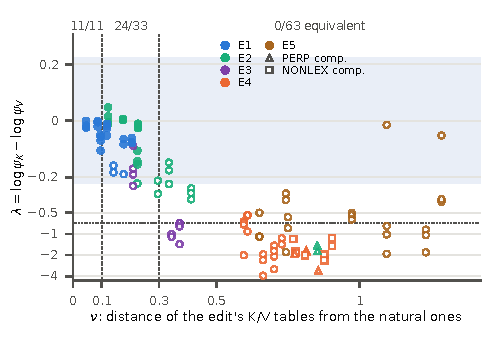
\includegraphics[width=0.62\textwidth]{figures/fig_nu.pdf}
\caption{\textbf{Post hoc: departures from the law follow how far an edit writes from the natural write.} Each point is one $\lambda$ statistic of an instance that carries identity ($\varphi$ without a mention at least 0.3), in the three models: full edits (circles; colour by family, E3 included although its gate failed) and PERP and NONLEX components (triangles, squares); filled: equivalent. $\nu$: the distance of the edit's cached keys and values from the natural ones, relative to the natural displacement. Band: $\pm\log 1.25$; dotted: $\log 0.5$, the copy-only bound; above the panel: equivalent of all statistics in each band of $\nu$ (cut-points chosen after the data). Linear $\nu$ axis; symmetric-log $\lambda$ axis, linear within $\pm 0.25$. Recomputed; post hoc.}
\label{fig:nu}
\end{figure}

\paragraph{Distance from the natural write (post hoc).} Over the \JcNuN{} $\lambda$ statistics of identity-carrying instances, $\lambda$ has Spearman correlation $\JcNuRhoNu$ with $\nu$ (95\,\% interval $\JcNuRhoNuLo$ to $\JcNuRhoNuHi$ from a bootstrap over the \JcNuUnits{} units of model, instance and depth, since each unit contributes several statistics) and \JcNuRhoCosK{} with the cosine of the edit's key displacement to the natural one; \JcNuEqLow{} of \JcNuNLow{} statistics with $\nu < 0.1$ are equivalent, \JcNuEqMid{} of \JcNuNMid{} with $\nu$ between 0.1 and 0.3, and \JcNuEqHigh{} of \JcNuNHigh{} beyond, of which \JcNuOutHigh{} have a 90\,\% interval wholly outside the margin (a shown departure) and the rest are inconclusive (\cref{fig:nu}). Four caveats limit the reading. (i)~The band cut-points 0.1 and 0.3 were chosen after the data. (ii)~At $\nu = 0$ the edit is the natural write and equivalence holds by construction, so a monotone association is partly guaranteed; only the rate of departure beyond small $\nu$ is informative. (iii)~$\nu$ is largely confounded with the edit family: of the \JcNuNBelow{} statistics with $\nu < 0.3$, \JcNuSteerBelow{} are steering vectors (E1, E2) and \JcNuEthreeBelow{} E3, while of the \JcNuNHigh{} beyond, \JcNuSteerAbove{} are steering vectors, \JcNuEthreeAbove{} E3 and \JcNuOtherAbove{} the remap, the non-lexical vectors and the components. Within the steering vectors ($n$ = \JcNuNSteer{}) the correlation is $\JcNuRhoSteer$; within the remap, non-lexical vectors and components ($n$ = \JcNuNOther{}) it is \JcNuRhoOther{}: beyond $\nu \approx 0.3$ every statistic comes from edits that are copy-read whatever their distance. (iv)~The table statistics are collinear (pairwise $\lvert$Spearman$\rvert$ \JcNuCollMin{}--\JcNuCollMax{} among $\nu$, the key, value and residual cosines and the first-order key projection), so $\nu$ cannot be told apart from the key cosine. The first-order prediction from the projections of the key and value displacements on the natural ones ranks the statistics only weakly (Spearman \JcOoneRho{}) and misses by $\JcOoneMiss$ on average: beyond $\nu \approx 0.3$ the key read collapses non-linearly while the value read decays more slowly (exploratory, recomputed). We therefore offer $\nu$ as a diagnostic to report alongside an intervention, not as an explanation of the departures. The pattern was found after the data and was not preregistered. A hypothesis for a future preregistration links it to the flag (\cref{app:flag}): the flag's dose response is threshold-like (half a flag barely moves the answer, one and two flags about equally), so the key route may select through a thresholded match while the value read degrades gradually; an edit that writes far from the natural state would then lose its key read first. It predicts that shrinking the key displacement of a near-natural steering vector past a threshold collapses $\psi_K$ while $\psi_V$ falls smoothly.

\paragraph{The key share against the natural share (reported).} At block 3 the steering vectors' key share is within 0.02 of the natural share in every format of all three models, while the remap's is lower. From block 3 to block 15 the change in the steering vectors' key share tracks the change in the natural share in \JcJcfourHold{} of \JcJcfourN{} qualifying pairs (largest gap \JcJcfourAbsMax{}), a consistency check that never enters the headline. % verbatim: "within 0.02", outcome J part C

\paragraph{Generated answers under the edits (exploratory).} At block 7, on the first 40 stories, E1 and E2 flip every generated answer without a mention in all three models, as the natural value does; with the options listed every edit flips fewer, the steering vectors at most as many as the natural value (natural value, E1, E2: \JcOfourOptNatQwenSeven{}, \JcOfourOptEoneQwenSeven{}, \JcOfourOptEtwoQwenSeven{} at Qwen2.5-7B; \JcOfourOptNatMistralSeven{}, \JcOfourOptEoneMistralSeven{}, \JcOfourOptEtwoMistralSeven{} at Mistral-7B; \JcOfourOptNatLlamaEight{}, \JcOfourOptEoneLlamaEight{}, \JcOfourOptEtwoLlamaEight{} at Llama-3.1-8B). The trained remap flips \JcOfourNoneEfouraQwenSeven{} / \JcOfourNoneEfouraMistralSeven{} and \JcOfourNoneEfourbQwenSeven{} / \JcOfourNoneEfourbMistralSeven{} of answers without a mention (two seeds; Qwen2.5-7B / Mistral-7B) but only \JcOfourOptEfouraQwenSeven{} / \JcOfourOptEfouraMistralSeven{} and \JcOfourOptEfourbQwenSeven{} / \JcOfourOptEfourbMistralSeven{} with the options listed: its key part, which the options' readers would need, is weak.
